
\subsection{Phonological generalizations}

\paragraph{Discovering phonological classes} Are CNLMs discovering distributional
generalizations about the phonological system of a language (as
noisily reflected in the orthography)? We
produced agglomerative clusterings of the
trained LSTM  input and output character embeddings. No clear pattern
emerged from the input embeddings, whereas the output
embeddings (probably more tuned to capture contextual dependencies)
led to meaningful phonological classes in all languages. This is illustrated for
German in Figure~\ref{fig:char-clustering}. We see a basic split
between vowels and consonants. Within the vowels, the front vowels
\emph{e} and \emph{i} cluster together. Within the consonants, we
observe a cluster of alveolar sonorants (\emph{n, l, r}). The
labial/labiodental \emph{f, p, b, v, w} plus intruder \emph{g}
form a cluster. Symbols often denoting velar or palatal sounds, such
as \emph{c}, \emph{k} and \emph{q} cluster together. The \emph{s} and \emph{{\ss}} letters, that, depending on context, denote the same
or closely related sounds, cluster together. While the
 clustering does not reflect a single,
consistent phonological dimension, it definitely suggests that the
CNLM has discovered a fair deal about the features organizing the
phonological system of the language.


% We conducted agglomerative clustering of character embeddings in the output layer.
% We found that, in all three languages, the highest-level clusters separated characters into consonants, vowels, numerals, punctuation, and various non-phonetic or rare characters.
% In Figure~\ref{fig:char-clustering}, we show a clustering of German character embeddings restricted to alphabetic characters.
% The top-level split partitions characters into vowels and consonants.
% %Parts of the finer clustering can be phonologically motivated, e.g., the liquids r, l form a cluster
% Consonant and vowel clusters each can, to a large extent, be phonologically motivated, though not along a single consistent dimensions:
% (TODO describe)
% %
% %Within the vowel cluster: in German, vowels and their fronted umlauts together (understandable as a consequence of morphological alternations), also e/i 
% %
% %Clustering of consonants can partly be motivated phonologically, though not along a single consistent dimensions:
% %In German, there are clusters sharing place of articulation (p/f, b/v/w, c/k/q). %, and the liquids (n/l/r) form a class 
% %

\begin{figure}
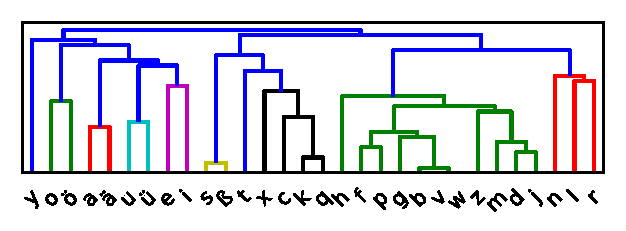
\includegraphics[width=0.50\textwidth]{figures/char-emb-clustering-output_output-phonetic-wiki-german-nospaces-bptt-910515909.pdf}
%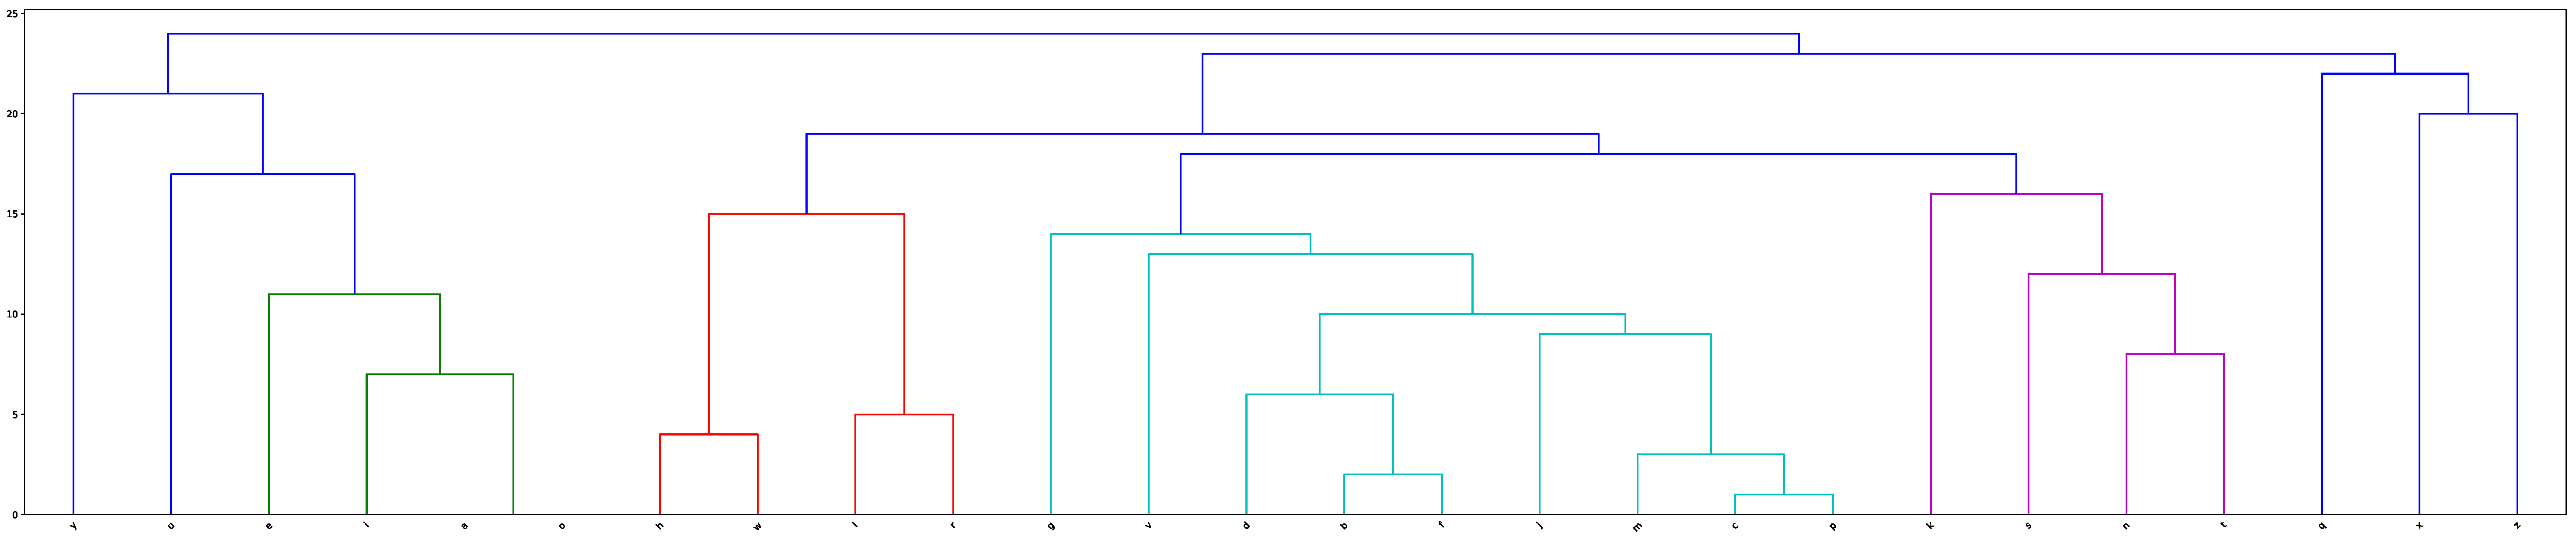
\includegraphics[width=0.48\textwidth]{figures/char-emb-clustering-output_output-phonetic-wiki-english-nospaces-bptt-282506230.pdf}
	%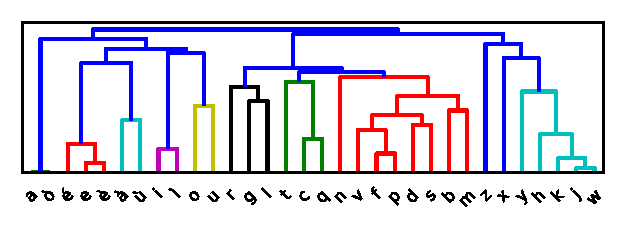
\includegraphics[width=0.48\textwidth]{figures/char-emb-clustering-output_output-phonetic-wiki-italian-nospaces-bptt-855947412.pdf}
\caption{Clustering of German character embeddings (alphabetic characters only)}\label{fig:char-clustering}
\end{figure}



\paragraph{Discovering phonotactic constraints}
\label{sec:phonotactics}

Next, we study whether the CNLM is capturing phonotactic constraints
more quantitatively.  We focus on German and Italian, as they
have reasonably transparent orthographies.  We construct pairs of
letter bigrams (picked to closely approximate phoneme bigrams) with
the same first letter, but such that one is phonotactically acceptable
in the language and the other isn't. We control letter frequencies
such that the independent unigram probability of the unacceptable
bigram is higher than that of the acceptable one. For example,
``\emph{br}'' is an acceptable Italian sequence and ``\emph{bt}''
isn't, although \emph{t} is more frequent than \emph{r}.  For each
such pair, we re-train the CNLMs on a version of the training partition
from which all words containing either bigram have been removed.  We
then look at the likelihood the re-trained model assigns to both sequences. If
the re-trained models systematically assign a larger probability to correct
sequences, this provides evidence that the CNLM implicitly possesses a
notion of phonological categories such as stops and sonorants, which
allows it to correctly generalize from attested sequences (e.g.,
``\emph{tr}'') to unattested ones (\emph{``br''}). In both languages,
we constructed two groups of bigrams: In one, the valid bigram had a
vowel following an obstruent; in the other, the obstruent was followed by
a liquid.  In both cases, in the invalid bigram, the obstruent was followed by a
stop or nasal.  % For each onset consonant and each of the two types, we
% considered valid vowels or sonorants satisfying the constraint on
% unigram frequencies, and randomly selected one if there were several.

Results are shown in Table \ref{tab:phonotactics-results} for all
bigram pairs (acceptable: left, impossible: right).  The LSTM assigns
higher probability to the acceptable bigrams in all but two cases.
This confirms that it has learnt about phonological categories such as
vowels and consonants and their phonotactic properties.  The
model makes the correct generalizations entirely on the basis of
distributional evidence, with no aid from perceptual or articulatory
cues. The RNN systematically prefers the impossible
bigrams, presumably because they have higher unigram probability. The
dramatic difference is surprising, since the relevant generalizations
pertain to adjacent symbols that either model should
capture. Possibly, although the tested rules are local, phonological
categories are better learnt by a model that can extract
generalizations about phoneme classes from wider contexts.

\begin{table}[t]
  \begin{small}
    \begin{center}
      \begin{tabular}{p{0.2cm}p{0.2cm}|p{0.6cm}p{0.6cm}||p{0.2cm}p{0.2cm}|p{0.99cm}p{0.8cm}}
        \multicolumn{4}{c||}{\emph{German}}   &       \multicolumn{4}{c}{\emph{Italian}}\\      \hline
        \multicolumn{2}{c}{\emph{}}&\emph{LSTM}&\emph{RNN} & \multicolumn{2}{c}{\emph{}}&  \emph{LSTM}&\emph{RNN}\\      \hline
        bu &  bt &  \textbf{ 4.6} &  0.2             &  bu & bd & \textbf{ $\approx$ 1} & $\approx$ 0 \\            
        do &  dd &  \textbf{ 1.9} &  0.1             &  du & dt & \textbf{ 1.3} & $\approx$ 0 \\             
        fu &  ft &  \textbf{ 6.5} &  $\approx$ 0             &  fu & ft & \textbf{ 30.5} & $\approx$ 0 \\             
        po &  pt &  \textbf{ 6.4} &  0.1             &  pu & pt & \textbf{ 6.8} & $\approx$ 0 \\             
        tu &  tt &  \textbf{ 5.4} &  $\approx$ 0             &  tu & td &  0.2 & $\approx$ 0 \\                       
        zu &  zt &  \textbf{ 2.4} &  0.2             &  vu & vd & \textbf{ 2.0} & $\approx$ 0 \\              \cline{1-4}
        bl &  bd &   0.8          & 0.2              &  zu & zt & \textbf{ 55.7} & $\approx$ 0 \\              \cline{5-8} 
        fl &  fd &  \textbf{ 2.1} & 0.8              &  br & bt & \textbf{ $\approx$ 1}  &  $\approx$ 0           \\ 
        fr &  fn &  \textbf{ 2.7} & 0.1              &  dr & dt & \textbf{ 2.5} & 0.4 \\               
        kl &  kt &  \textbf{ 3.8} & 0.1              &  fr & ft & \textbf{ 2.9} & $\approx$ 0 \\             
        pl &  pt &  \textbf{ 2.5} & 0.9              &  pr & pt & \textbf{ 5.0} & $\approx$ 0 \\              \hline
        \multicolumn{2}{c|}{AM}      & \textbf{3.6} & 0.2     & 	    \multicolumn{2}{c|}{AM}   & \textbf{10.7}  & $\approx$ 0         \\
        \multicolumn{2}{c|}{GM} & \textbf{3.0} & 0.1          & 	    \multicolumn{2}{c|}{GM}   & \textbf{3.2} & $\approx$ 0           \\

%                     bu &  bt &  \textbf{ 4.6} &  0.22             &  bu & bd & \textbf{ 1.001} & 6e-5 \\            
%                     do &  dd &  \textbf{ 1.9} &  0.05             &  du & dt & \textbf{ 1.3} & 0.008 \\             
%                     fu &  ft &  \textbf{ 6.5} &  0.03             &  fu & ft & \textbf{ 30.5} & 0.01 \\             
%                     po &  pt &  \textbf{ 6.4} &  0.10             &  pu & pt & \textbf{ 6.8} & 0.008 \\             
%                     tu &  tt &  \textbf{ 5.4} &  0.02             &  tu & td &  0.2 & 3e-5 \\                       
%		     zu &  zt &  \textbf{ 2.4} &  0.17             &  vu & vd & \textbf{ 2.0} & 2e-5 \\              \cline{1-4}
%                     bl &  bd &   0.8          & 0.18              &  zu & zt & \textbf{ 55.7} & 0.01 \\              \cline{5-8} 
%                     fl &  fd &  \textbf{ 2.1} & 0.82              &  br & bt & \textbf{ 1.001}  &  0.006           \\ 
%                     fr &  fn &  \textbf{ 2.7} & 0.10              &  dr & dt & \textbf{ 2.5} & 0.4 \\               
%                     kl &  kt &  \textbf{ 3.8} & 0.10              &  fr & ft & \textbf{ 2.9} & 0.001 \\             
%                     pl &  pt &  \textbf{ 2.5} & 0.86              &  pr & pt & \textbf{ 5.0} & 0.008 \\              \hline
%	    \multicolumn{2}{c|}{AM}      & \textbf{3.6} & 0.24     & 	    \multicolumn{2}{c|}{AM}   & \textbf{10.7}  & 0.041          \\
%	    \multicolumn{2}{c|}{GM} & \textbf{3.0} & 0.13          & 	    \multicolumn{2}{c|}{GM}   & \textbf{3.2} & 0.0021           \\

      \hline
    \end{tabular}
  \end{center}    
  \end{small}
	\caption{\label{tab:phonotactics-results} Likelihood ratio between acceptable and unacceptable bigrams, with arithmetic (AM) and geometric (GM) means. Values $>1$ in bold.}
\end{table}
